\section{Rigid versus soft curb}\label{sec:compare}

\Cref{tab:compare} lists the slot lengths in both models for the six cars of \cref{tab:cars}, and \cref{fig:compare} plots them for the typical car.
By \eqref{eq:soft-le} no soft-curb value can exceed the corresponding rigid-curb value, and the computed values respect this.

\begin{table}[ht]
\centering\small
\begin{tabular}{@{}llccccc@{}}
\toprule
car & curb & $n=1$ & $n=2$ & $n=3$ & $n=4$ & $n=5$\\
\midrule
City car & rigid & 4.910 & 4.517 & 4.311 & 4.222 & 4.132\\
 & soft & 4.895 & 4.471 & 4.277 & 4.189 & 4.128\\
\addlinespace[2pt]
Compact & rigid & 5.686 & 5.271 & 5.126 & 5.024 & 4.911\\
 & soft & 5.664 & 5.186 & 4.971 & 4.872 & 4.815\\
\addlinespace[2pt]
Typical & rigid & 5.833 & 5.411 & 5.280 & 5.180 & 5.050\\
 & soft & 5.809 & 5.312 & 5.088 & 4.978 & 4.906\\
\addlinespace[2pt]
Mid-size sedan & rigid & 6.452 & 6.052 & 5.926 & 5.844 & 5.744\\
 & soft & 6.419 & 5.866 & 5.621 & 5.507 & 5.433\\
\addlinespace[2pt]
Large SUV & rigid & 6.877 & 6.393 & 6.288 & 6.187 & 6.069\\
 & soft & 6.840 & 6.231 & 5.959 & 5.831 & 5.758\\
\addlinespace[2pt]
Van & rigid & 7.543 & 6.969 & 6.850 & 6.734 & 6.597\\
 & soft & 7.503 & 6.794 & 6.480 & 6.330 & 6.253\\
\bottomrule
\end{tabular}
\caption{Slot lengths (in metres) with a rigid curb (\cref{tab:cars}) and with a soft curb, for margin $m=w/10$ and the tyre data of \cref{sec:model-soft}.
For $n=1$ the values are exact (\cref{thm:one,thm:one-soft}; for the city car the soft value is numerical).
For $n=2$ the soft values are $\Lambda_2^{\rm s}$ of \cref{prop:two-soft}; all entries with $n\ge2$ are upper bounds.}
\label{tab:compare}
\end{table}


\begin{figure}[ht]
\centering
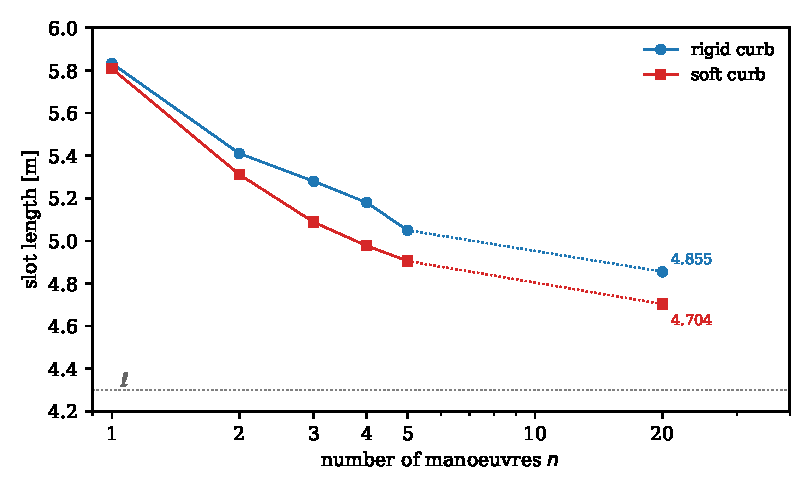
\includegraphics[width=0.8\textwidth]{figures/fig_compare.pdf}
\caption{Slot lengths with $n$ manoeuvres for the typical car, with a rigid curb (blue) and a soft curb (red).
The values for $n=1$ are exact; the others come from explicit strategies and are upper bounds.
The dotted segments only join $n=5$ to $n=20$.}
\label{fig:compare}
\end{figure}

\paragraph{One manoeuvre.}
The optimal single manoeuvres have the same shape in both models.
The car starts tilted nose-up, as far back and as high as possible, and drives out with full left lock while its front curb-side corner grazes $\Qf$.
Both slot lengths are values of the same function, $\Lmin(1)=\varphi_0(\psi_d)$ and $\Lmins(1)=\varphi_0(\psi_t)$; only the admissible tilt differs.
With a rigid curb the tilt is limited by the swing of the rear corner towards the curb during the turn.
With a soft curb the rear corner may pass over the curb, and the tilt is limited by the rear tyre touching the curb at rest.
The gain is small, $1.5$--$3.9$ cm for our six cars, because in both models the decisive constraint is the corner $\Qf$ of the car in front.
Both values are below the classical length $d_b+\sqrt{b^2+2Rw}$, by $2.8$ and $5.3$ cm for the typical car.

\paragraph{Two manoeuvres.}
Here the curb matters much more.
With a soft curb the textbook exit of \cref{prop:two-soft} is admissible: reverse with full right lock until the rear bumper touches the car behind, then leave with full left lock.
Its length $\Lambda_2^{\rm s}$ depends neither on the margin nor on the tyres.
With a rigid curb this exit would drive the rear corner into the curb.
The best rigid exit we know (\cref{prop:two-better}) therefore first turns the car slightly nose-down and needs three contacts.
The soft curb saves between $4.6$ and $18.6$ cm, and $9.9$ cm for the typical car.

\paragraph{Three to twenty manoeuvres.}
The rotation zigzags work in both models, but they are limited by different contacts.
With a rigid curb each reverse manoeuvre ends when the rear corner meets the curb.
With a soft curb it ends when the rear bumper meets the car behind.
For three to five manoeuvres the best soft-curb zigzags we found are $14$--$20$ cm shorter than the rigid-curb ones for the typical car, and up to about $40$ cm shorter for the van.
In \cref{tab:compare} the gain roughly grows with the rear overhang, the part of the car that swings towards the curb when it reverses: it is largest for the mid-size sedan, the large SUV and the van ($d_b\ge1$ m) and only a few centimetres for the city car ($d_b=0.55$ m).
With twenty manoeuvres the typical car needs $4.704$ m instead of $4.855$ m, and its motion is wedged between the two parked cars instead of between the curb and the car in front (\cref{app:twenty-soft,app:twenty}); the five-manoeuvre motions of \cref{app:five-soft,app:five} differ in the same way.

\paragraph{Many manoeuvres.}
By \cref{prop:asym-soft}, $\sqrt n\,(\Lmin(n)-\ell)$ and $\sqrt n\,(\Lmins(n)-\ell)$ have the same limit $K$.
Hence the ratio of the slacks $\Lmins(n)-\ell$ and $\Lmin(n)-\ell$ tends to $1$.
For large $n$ the car stays nearly level while it crawls out, its lowest point stays near the height $m$, and the curb plays no role.

\paragraph{The margin.}
With a rigid curb a positive margin is indispensable: for $m=0$ no slot length suffices (\cref{prop:flush}).
With a soft curb the flush problem is well posed, and for the typical car one manoeuvre then needs $5.856$ m.
A positive margin still helps: it allows a larger tilt of the starting position in \cref{thm:one-soft} ($\psi_t=0.0561$ instead of $0.0073$ rad for the typical car) and the two-manoeuvre exit of \cref{prop:two-soft}.

\paragraph{Which model applies?}
The soft-curb model describes a curb that the overhangs of the car can clear, with nothing behind it that they could hit.
In our motions the body passes at most $9$ cm beyond the curb for the typical car, and about $15$ cm for the largest cars.
The rigid-curb model describes a wall, or a curb too high for the overhangs.
For one manoeuvre the distinction is nearly irrelevant, since the two values differ by a few centimetres.
For two to five manoeuvres it is worth up to $40$ cm, depending on the car, and drivers who know that their overhangs clear the curb can use correspondingly shorter gaps.

\paragraph{Sensitivity to the tyre data.}
Our tyre data are typical values, not measurements of particular cars.
The two-manoeuvre value $\Lambda_2^{\rm s}$ does not depend on them, as long as \ref{T:tyre} and \ref{T:end} hold.
For the typical car the one-manoeuvre value changes by less than $1.6$ cm when $\delta_s$ ranges over $[0,5]$ cm and $\lambda$ over $[0.20,0.30]$ m: it stays between $5.802$ and $5.817$ m (\texttt{numerics/soft\_sens.py}).
For some of these tyres \cref{ass:soft} fails; there the numerical optimum exceeds $\varphi_0(\psi_t)$ by at most $0.2$ mm, as for the city car.
The multi-manoeuvre motions keep the tyres well away from the curb: for the six cars at least $6.7$ cm with two manoeuvres and at least $11$ cm with three to five.
They all remain free for the largest tyres of this range, $\delta_s=0$ and $\lambda=0.30$ m (\cref{app:numerics}).
Since the lowest tyre point moves down as $\lambda$ grows or $\delta_s$ shrinks, all our upper bounds with $n\ge2$ hold for every choice of tyre data in this range.
